% Original neuron-level template. Change the layer list in BOTH loops together.
\documentclass[tikz,border=10pt]{standalone}
\usepackage[T1]{fontenc}
\usepackage{lmodern,amsmath}
\usetikzlibrary{arrows.meta}
\definecolor{ink}{HTML}{14263D}
\definecolor{blue}{HTML}{2563EB}
\definecolor{violet}{HTML}{6D28D9}
\definecolor{teal}{HTML}{0F766E}
\begin{document}
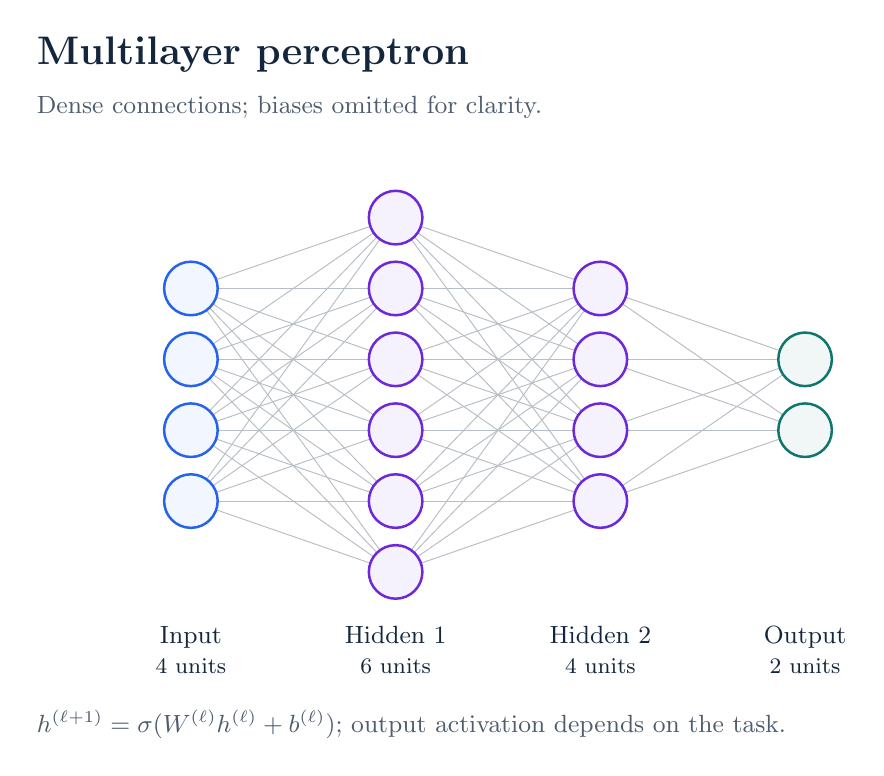
\begin{tikzpicture}[font=\sffamily,text=ink,x=26mm,y=9mm]
\node[anchor=west,font=\Large\bfseries] at (-.8,4.8) {Multilayer perceptron};
\node[anchor=west,font=\small,text=ink!75] at (-.8,4.05) {Dense connections; biases omitted for clarity.};
% Draw edges first so neuron outlines remain clear.
\foreach \layer/\units/\previous in {1/6/4,2/4/6,3/2/4}{
  \pgfmathtruncatemacro{\prevlayer}{\layer-1}
  \foreach \i in {1,...,\previous}{
    \foreach \j in {1,...,\units}{
      \draw[ink!30,line width=.35pt] (\prevlayer,{(\previous+1)/2-\i}) -- (\layer,{(\units+1)/2-\j});
    }
  }
}
\foreach \layer/\units/\clr/\label in {0/4/blue/Input,1/6/violet/Hidden 1,2/4/violet/Hidden 2,3/2/teal/Output}{
  \foreach \i in {1,...,\units}{
    \node[circle,draw=\clr,fill=\clr!6,line width=.9pt,minimum size=6.8mm,inner sep=0] at (\layer,{(\units+1)/2-\i}) {};
  }
  \node[align=center,font=\small] at (\layer,-3.6) {\label\\\footnotesize\units\ units};
}
\node[anchor=west,font=\small,text=ink!75] at (-.8,-4.65) {$h^{(\ell+1)}=\sigma(W^{(\ell)}h^{(\ell)}+b^{(\ell)})$; output activation depends on the task.};
\end{tikzpicture}
\end{document}
